\definecolor{NPSS}{HTML}{00D0FF}
\definecolor{NSSS}{HTML}{F97BFF}
\definecolor{NPBCH}{HTML}{92D050}
\usetikzlibrary{patterns,decorations.pathreplacing}

\resizebox{\textwidth}{!}{
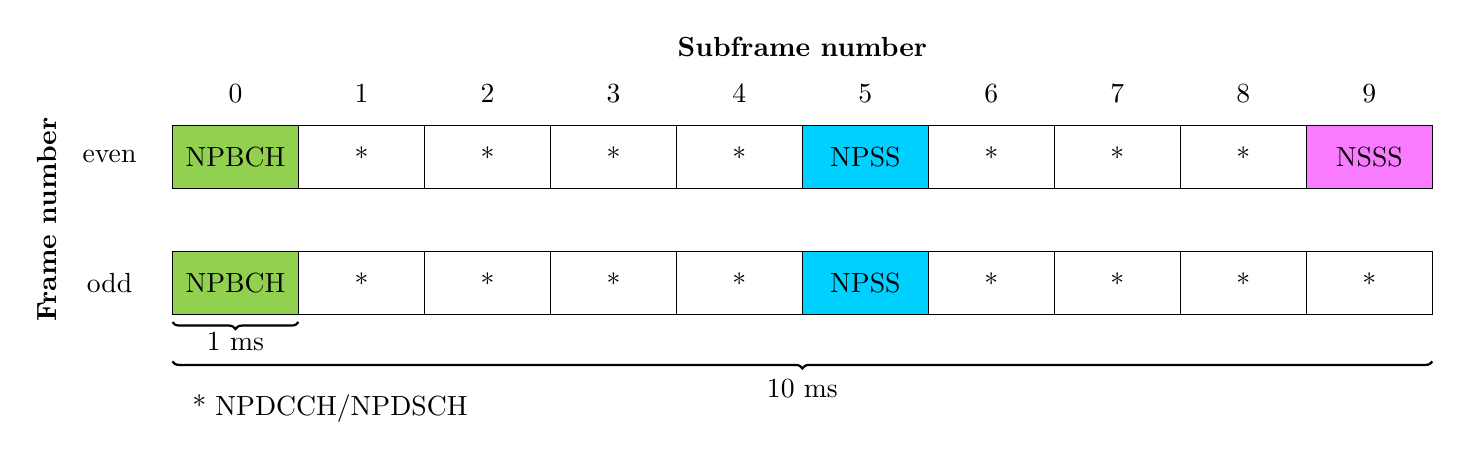
\begin{tikzpicture}[scale = 0.4]

\draw [thick,decoration={brace,mirror,raise=0.1cm},decorate] (-20,-4) -- (-16,-4) node [pos=0.5,anchor=north,yshift=-0.1cm] {1 ms}; 
\draw [thick,decoration={brace,mirror,raise=0.2cm},decorate] (-20,-5) -- (20,-5) node [pos=0.5,anchor=north,yshift=-0.3cm] {10 ms};



\draw[fill = NPBCH]  (-20,2) rectangle (-16,0);
\draw  (-16,2) rectangle (-12,0);
\draw  (-12,2) rectangle (-8,0);
\draw  (-8,2) rectangle (-4,0);
\draw  (-4,2) rectangle (0,0);
\draw[fill = NPSS]  (0,2) rectangle (4,0);
\draw  (4,2) rectangle (8,0);
\draw  (8,2) rectangle (12,0);
\draw  (12,2) rectangle (16,0);
\draw[fill = NSSS]  (16,2) rectangle (20,0);

\draw[fill = NPBCH]  (-20,-2) rectangle (-16,-4);
\draw  (-16,-2) rectangle (-12,-4);
\draw  (-12,-2) rectangle (-8,-4);
\draw  (-8,-2) rectangle (-4,-4);
\draw  (-4,-2) rectangle (0,-4);
\draw[fill = NPSS]  (0,-2) rectangle (4,-4);
\draw  (4,-2) rectangle (8,-4);
\draw  (8,-2) rectangle (12,-4);
\draw  (12,-2) rectangle (16,-4);
\draw  (16,-2) rectangle (20,-4);

\node at (-18,3) {0};
\node at (-14,3) {1};
\node at (-10,3) {2};
\node at (-6,3) {3};
\node at (-2,3) {4};
\node at (2,3) {5};
\node at (6,3) {6};
\node at (10,3) {7};
\node at (14,3) {8};
\node at (18,3) {9};
\node at (-22,1) {even};
\node at (-22,-3) {odd};
\node [rotate = 90] at (-24,-1) {\textbf{Frame number}}; 

\node at (-18,1) {\acrshort{NPBCH}};
\node at (-18,-3) {\acrshort{NPBCH}};
\node at (2,1) {\acrshort{NPSS}};
\node at (2,-3) {\acrshort{NPSS}};
\node at (18,1) {\acrshort{NSSS}};
\node at (-14,1) {*};
\node at (-10,1) {*};
\node at (-6,1) {*};
\node at (-2,1) {*};
\node at (6,1) {*};
\node at (10,1) {*};
\node at (14,1) {*};
\node at (-14,-3) {*};
\node at (-10,-3) {*};
\node at (-6,-3) {*};
\node at (-2,-3) {*};
\node at (6,-3) {*};
\node at (10,-3) {*};
\node at (14,-3) {*};
\node at (18,-3) {*};
\node at (0,4.5) {\textbf{Subframe number}}; 

\node at (-15,-7) {* \acrshort{NPDCCH}/\acrshort{NPDSCH}};
\end{tikzpicture}
}
